\documentclass[12pt]{article}
\usepackage[margin=1in]{geometry}
% \usepackage[scaled]{helvet}
% \renewcommand{\familydefault}{\sfdefault}  % Use sans-serif as default
\usepackage{float}
\usepackage{array}
\usepackage{caption}
\usepackage{amsmath}
\usepackage{hyperref}
\usepackage{pdflscape}
\usepackage{afterpage}
\hypersetup{
    colorlinks=true,
    linkcolor=black,
    citecolor=black,
    urlcolor=black
}
\usepackage{graphicx}
\usepackage{tocloft}  % Optional: improves TOC formatting
\usepackage{acronym}  % For acronyms
\setlength{\parindent}{0pt}
\usepackage{multirow}
\usepackage{longtable}
\usepackage{makecell}
\usepackage{natbib}
\usepackage{sectsty}

% Set all section headings to 12pt AND bold
% \sectionfont{\fontsize{12}{14}\selectfont\bfseries}
% \subsectionfont{\fontsize{12}{14}\selectfont\bfseries}
% \subsubsectionfont{\fontsize{12}{14}\selectfont\bfseries}

\bibliographystyle{chicago}

\renewcommand{\arraystretch}{1.5} % Increases row height slightly for clarity
\newcolumntype{C}[1]{>{\centering\arraybackslash}m{#1}}  % centered horizontally and vertically


\begin{document}

\title{L'SPACE Mission Concept Review\\\large Team 18: Vitalis}
\author{}
\date{}

\maketitle 
\begin{center}
\begin{minipage}{0.45\linewidth}
    \centering
    
\includegraphics[width=0.9\linewidth]{images/newvitalis.png}
\end{minipage}%
\hspace{0.05\linewidth}
\begin{minipage}{0.45\linewidth}
    \centering
    
\includegraphics[width=0.9\linewidth]{images/nasa.png}
\end{minipage}
\end{center}


\vspace{2em}

\noindent
\begin{center}
\begin{minipage}{\textwidth}
\centering
\vspace{10em}
\textbf{\Large Team Members}

\vspace{2em}

\begin{tabular}{>{\centering\arraybackslash}p{0.95\textwidth}}
\textbf{Sara John} \\ 
\small Project Manager \\
\begin{tabular}{>{\centering\arraybackslash}p{0.3\textwidth} >{\centering\arraybackslash}p{0.3\textwidth} >{\centering\arraybackslash}p{0.3\textwidth}}
\textbf{Loqain Ahmed} & \textbf{Charlie Westwood} & \textbf{Daniel Parachalla} \\
\small Chief Scientist & \small Lead Systems Engineer & \small Deputy PM of Resources \\
\end{tabular} \\[1em]
\begin{tabular}{>{\centering\arraybackslash}p{0.3\textwidth} >{\centering\arraybackslash}p{0.3\textwidth} >{\centering\arraybackslash}p{0.3\textwidth}}

\textbf{Triston Lindsrois} & \textbf{Isaly Rodriguez} & \textbf{Juan Alvarez} \\
\small Astrobiologist & \small Mechanical Eng. (PL) & \small Program Analyst \\

\textbf{Ryan Collingham} & \textbf{Reesa Mathew} & \textbf{Shruthi Anantharajan} \\
\small Astrobiologist & \small Mechanical Eng. (PG) & \small Program Analyst \\

\textbf{Mann Patel} & \textbf{Meghan Prince} & \textbf{Reesa Mathew} \\
\small Planetary Geologist & \small Electrical Eng. (PL) & \small Mission Assurance Specialist \\

\textbf{Albert Bermingham} & \textbf{Damian Micor} & \textbf{Hannah Parisella} \\
\small Planetary Geologist & \small Electrical Eng. (PG) & \small Mission Assurance Specialist \\

& \textbf{Ahmed Yousef} & \\
& \small Thermal Eng. (PL) & \\

& \textbf{Isabella Schroeder} & \\
& \small Thermal Eng. (PG) & \\

& \textbf{Kaden Chen} & \\
& \small Comp. Hardware Eng. (PL) & \\

& \textbf{Ferdows Alriashi} & \\
& \small Comp. Hardware Eng. (PG) & \\

\end{tabular}
\end{tabular}
\end{minipage}
\end{center}

\clearpage

% Table of Contents
\tableofcontents
\clearpage

% Table of Figures
\listoffigures
\clearpage

% Table of Acronyms
\section*{Table of Acronyms}
\begin{acronym}[SWIM] % Longest acronym here for spacing
  \acro{CDH}{Command and Data Handling}
  \acro{CDR}{Critical Design Review}
  \acro{COSPAR}{Committee on Space Research}
  \acro{CRISM}{Compact Reconnaissance Imaging Spectrometer for Mars}
  \acro{EDL}{Entry, Descent, and Landing}
  \acro{EZ}{Exploration Zone}
  \acro{GCR}{Galactic Cosmic Rays}
  \acro{GPR}{Ground Penetrating Radar}
  \acro{HBS}{Human and Biological Science}
  \acro{ISRU}{In-Situ Resource Utilization}
  \acro{JMARS}{Java Mission-planning and Analysis for Remote Sensing}
  \acro{L’SPACE}{Lucy Student Pipeline Accelerator and Competency Enabler}
  \acro{MEPAG}{Mars Exploration Program Analysis Group}
  \acro{MRO}{Mars Reconnaissance Orbiter}
  \acro{NS}{Neutron Spectrometer}
  \acro{PDR}{Preliminary Design Review}
  \acro{PL}{Payload Lead}
  \acro{PG}{Programmatics Group}
  \acro{PPM}{Parts Per Million}
  \acro{SEP}{Solar Energetic Particles}
  \acro{STM}{Science Traceability Matrix}
  \acro{SWIM}{Subsurface Water Ice Mapping}
  \acro{TBD}{To Be Determined}
  \acro{TBR}{To Be Resolved}
  \acro{TIR}{Thermal Infrared Spectrometer}
  \acro{VNIR}{Visible and Near Infrared}
\end{acronym}
\clearpage


% Main content
\section*{1.1 Mission Statement}
\addcontentsline{toc}{section}{1.1 Mission Statement}

The goal of this mission is to detect and characterize near-surface water ice within a high-priority Exploration Zone (EZ) on Mars. This effort aims to enable both breakthrough scientific discoveries and to support NASA's long-term objective of sustained human presence on the Red Planet. Specifically, the mission will gather geophysical and compositional data related to shallow subsurface water ice (0–1 meter depth) and associated hydrated minerals. This data is crucial for evaluating in situ resource availability, assessing potential habitability, and reducing risk for future crewed missions. \\

To accomplish this, the mission will deploy a lightweight, solar-powered robotic rover equipped with a suite of instruments capable of in situ analysis. The rover will traverse a 10 km × 10 km region, targeting diverse terrain types such as impact craters, polygonal ground, and sloped regolith to maximize the probability of detecting preserved ice. Key payload instruments include ground-penetrating radar to detect dielectric contrasts linked to ice layers, neutron spectroscopy for hydrogen abundance mapping, and visible/infrared spectrometers for mineralogical context. \\

In addition to scientific instrumentation, the rover will carry a compact, human-exploration-relevant astrobiology experiment. This experiment, constrained by mass and volume limitations, will test life detection protocols or contamination mitigation strategies directly applicable to future crewed exploration. \\

The collected data will enhance our understanding of the Martian cryosphere, inform models of planetary climate evolution, and directly support site selection for In-Situ Resource Utilization (ISRU). This mission will serve as a key stepping stone toward NASA’s Moon to Mars exploration architecture by providing actionable data for landing site assessment, resource extraction, and long-duration surface operations. \\
\section*{1.2 Science Traceability Matrix (STM)}
\addcontentsline{toc}{section}{1.2 Science Traceability Matrix (STM)}

This mission addresses one of the most compelling questions in planetary science and astrobiology: \textit{What are the long-term endogenic and exogenic controls on the presence of liquid water on terrestrial planets?} (Decadal Survey Q10.3b)\footnote{See \cite{nrc_2022_decadal}}. The team's concept, a lightweight robotic rover that targets mid-latitudes of Mars, is strategically designed to explore the interaction between Mars's internal geologic processes, external climatic forces, and the current distribution and persistence of water ice. The mission supports robotic and human exploration, meeting the highest priority stakeholder needs outlined in NASA’s Mission Task Document and Decadal Strategy\footnote{See \cite{lspace_stm_module, mepag_goals}}. \\

The science traceability process began with a detailed examination of the Q10.3b prompt, followed by the derivation of two mission-specific science exploration objectives, and two human exploration objectives. The first objective focuses on the detection and geophysical characterization of subsurface water ice, while the second targets understanding how geological and climatic history influence the ice’s stability, location, and potential habitability. These objectives are aligned with the strategic needs for Mars exploration, particularly in evaluating possible human landing sites and long-term outpost support\footnote{See \cite{nasa_m2m_objectives}}. \\

The traceability matrix baselines the first three columns, science goals, objectives, and measurements, ensuring a clear, logical flow from high-level priorities to mission implementation. Subsequent columns include physical parameters, observables, performance requirements, instruments, and mission constraints. All measurements are designed to be feasible within the constraints of a Discovery-class rover profile (≤200 kg, ≤2.5 m\textsuperscript{3}, ≤\$450M). \\

\subsection*{Science Objective 1: Detect Subsurface Water Ice}

The primary method for identifying subsurface ice is radar sounding, executed via a forward-facing ground-penetrating radar modeled after SHARAD and RIMFAX\footnote{See \cite{plaut_2007_subsurface, putzig_2012_stratigraphy}}. This instrument can detect dielectric interfaces corresponding to water ice layers up to 10 meters deep. Complementary to this, a neutron spectrometer—derived from DAN or NS can passively detect hydrogen signatures as indirect indicators of water presence\footnote{See \cite{nasa_rad}}. Together, these instruments could provide volumetric and compositional data at decimeter-scale resolution. \\

To provide further context, surface spectrometers (VNIR or TIR) can identify hydrated minerals such as perchlorates and sulfates, offering insights into historical water-rock interactions. In Moreux Crater, glacial features and lobate debris aprons can be linked to mineralogical evidence of past ice movement and melting\footnote{See \cite{bramson_2015_excess, mellon_1995_ground_ice}}.

\subsection*{Science Objective 2: Understand Controls on Water Distribution}

Identifying water is only the first step— understanding its distribution and stability is critical. This objective requires integrating geological and climatic data. The rover will assess regolith thermal properties, atmospheric pressure, and diurnal temperature cycles to determine whether detected ice is currently stable or a remnant of past epochs. Subsurface temperature gradients will be inferred via thermal inertia modeling and validated with onboard environmental sensors. \\

Topographic and geomorphological mapping with stereo cameras and radar will reveal how crater slopes, elevation, and insulating regolith thickness influence ice preservation. By correlating observed ice depths with geologic unit boundaries, the mission will identify controlling factors such as lithologic variation or glacial resurfacing\footnote{See \cite{head_2010_glaciation}}. \\

These findings directly support ISRU planning, inform site safety for future human landings, and contribute to broader planetary evolution models. Whether subsurface ice is stable over decadal timescales or sensitive to obliquity-driven changes will critically affect the sustainability of surface infrastructure on Mars.

\subsection*{Stakeholder Satisfaction}

This STM supports both robotic science and exploration readiness. All objectives align with the Decadal Survey, MEPAG goals, and the Mission Task\footnote{See \cite{nrc_2022_decadal, mepag_goals, lspace_stm_module}}. The mission will produce high-value data to inform the selection of future crewed landing sites by resolving key questions about water accessibility and environmental stability. The STM is fully baselined, with TBDs limited to instrument performance parameters or mission requirement margins—each to be addressed in the TBD/TBR Resolution Table.




\begin{table}[H]
\caption{Science Traceability Matrix (STM)}
\hspace{-1cm}
\scalebox{1.1}{
\renewcommand{\arraystretch}{1.5}
\scriptsize
\resizebox{\textwidth}{!}{%
\begin{tabular}{|C{4cm}|C{4cm}|C{4.5cm}|C{4cm}|C{3cm}|C{2.5cm}|C{2.5cm}|C{2.2cm}|C{2.2cm}|}
\hline
\textbf{Science Goals} & \textbf{Science Objectives} & \textbf{Physical Parameters} & \textbf{Observables} & \textbf{Science Measurement Requirements} & \textbf{Instrument Performance Requirements} & \textbf{Predicted Instrument Performance} & \textbf{Instrument} & \textbf{Mission Requirements} \\
\hline

\multirow{3}{=}{{HBS-1LM: Understand the effects of short- and long-duration exposure to the environments of the Moon, Mars, and deep space on biological systems and health, using humans, model organisms, systems of human physiology, and plants.}} 
& Determine the impact of Martian dust on human respiratory systems by characterizing the toxicity, particle size distribution, and chemical composition of airborne particles. 
& Identify if hexavalent Chromium is present in Martian soil and airborne dust at more than 150 ppm & Collect UV-visible absorbance spectra between 350–450 nm from soil and airborne dust samples processed every 6 solar hours. & TBD 1 & TBD 2 & TBD 5 & TBD 6 & TBD 9 \\
\cline{2-9}
& Assess the radiation environment and its effects on biological systems by measuring cosmic ray flux and cumulative dose rates at the Martian surface.
& Determine the cumulative radiation dose absorbed by phantom lung tissue over a 50-sol period on the Martian surface, including radiation contributions from GCR and solar particle events. & Quantify the energy deposition rate and flux of ionizing radiation in particles/cm²/s in phantom tissues across a 10 MeV-1 GeV range, with data collected hourly. & TBD 1 & TBD 2 & TBD 5 & TBD 6 & TBD 9 \\
\hline

\multirow{2}{=}{{Q10.3b: What are the long-term endogenic and exogenic controls on the presence of liquid water on terrestrial planets?}} 
& Determine if there is liquid water on or near the surface through geochemical measurements of ice and hydrous minerals and geophysical measurements of the crust.
& Identify the presence of water-bearing minerals, including Fe/Mg and Al-rich phyllosilicates and sulfates, in surface and near-surface regolith within a 100 m² study area.  & Measure reflectance spectra between 1.9–2.5 µm with mineral abundances resolved at a spatial resolution of 1 m. & TBD 3 & TBD 4 & TBD 7 & TBD 8 & TBD 10 \\
\cline{2-9}
& Determine the distribution, history, and processes driving the availability of ice and liquid water.
& Determine spatial variability in the deuterium-to-hydrogen (D/H) ratio of subsurface ice to assess contributions from distinct ancient water reservoirs and the regional history of water loss (Cockell, et all 2016). & Measure isotopic ratios of H and D in vapors released from subsurface ice at 5-meter lateral intervals, with a resolution of 0.1‰ & TBD 3 & TBD 4 & TBD 7 & TBD 8 & TBD 10 \\
\hline

\end{tabular}
}}
\end{table}




\section*{1.3 Summary of Mission Location}
\addcontentsline{toc}{section}{1.3 Summary of Mission Location}

Mars, the fourth planet from the Sun, is a cold, terrestrial world with a thin carbon dioxide (CO\textsubscript{2}) atmosphere\footnote{See \cite{asu_2019_atmosphere}}. Its surface is shaped by volcanic activity, impact cratering, aeolian erosion, and seasonal freeze-thaw processes. The planet experiences extreme temperature variations, frequent dust storms, and high radiation levels due to the absence of a global magnetic field and protective upper atmosphere. Despite these challenges, Mars remains a prime candidate for exploration, largely because of its potential to harbor accessible water ice in the near subsurface\footnote{See \cite{nrc_2022_decadal}}.\\

Orbital datasets from missions such as Mars Odyssey, the Mars Reconnaissance Orbiter (MRO), and the Subsurface Water Ice Mapping (SWIM) project have revealed compelling evidence of near-surface hydrogen-rich regolith in the northern mid-latitudes. These regions are believed to contain water ice at depths of less than one meter—ideal for both scientific investigation and in situ resource utilization (ISRU) in support of future human missions\footnote{See \cite{bramson_2015_excess, mellon_1995_ground_ice}}. The latitude range also offers favorable thermal conditions and sufficient solar availability for rover operations.\\

This mission targets a 10 km × 10 km Exploration Zone (EZ) located within one of NASA’s high-priority shallow ice candidate zones, as defined by the SWIM maps. The region will be selected based on three key criteria:

\begin{itemize}
    \item Presence of subsurface water ice at 0–1 m depth
    \item Geologic features indicative of volatile exposure or preservation
    \item Navigable terrain within rover mobility and risk constraints
\end{itemize}

Candidate features within the EZ may include:

\begin{itemize}
    \item \textbf{Recent impact craters} — may expose subsurface volatiles via fresh ejecta\footnote{See \cite{bramson_2015_excess}}
    \item \textbf{Polygonal terrain} — indicates thermal contraction and seasonal freeze-thaw cycles\footnote{See \cite{mellon_1995_ground_ice}}
    \item \textbf{Gently sloped surfaces} — improve rover stability and may help preserve underlying ice
    \item \textbf{Spectral signatures from CRISM and SHARAD} — suggest hydrated minerals or water-bearing deposits\footnote{See \cite{plaut_2007_subsurface, putzig_2012_stratigraphy, nasa_sharad_data}}
\end{itemize}

Site selection will be finalized using NASA’s JMARS (Java Mission-planning and Analysis for Remote Sensing) tool, informed by overlays from SWIM, CRISM mineralogical maps, elevation models, and slope data. Final considerations will include engineering feasibility, astrobiological interest, planetary protection constraints, and accessibility for surface mobility\footnote{See \cite{head_2010_glaciation}}.\\

Targeting this terrain directly advances NASA’s Moon to Mars objectives and the Mars Exploration Program Analysis Group (MEPAG) science goals by identifying accessible water resources for ISRU, while also informing future long-duration surface operations and life-detection strategies\footnote{See \cite{nrc_2022_decadal}}.

\section*{1.4 Mission Requirements}
\addcontentsline{toc}{section}{1.4 Mission Requirements}

The mission requirements are derived directly from the science and exploration objectives, the customer-imposed constraints outlined in the Mission Task Document, and the environmental conditions expected on the Martian surface. These requirements serve as concrete, measurable benchmarks for mission success and help define the design envelope for each subsystem.
\\
To meet its objectives, the mission must balance scientific return with strict engineering limitations, including mass, volume, power architecture, and cost. The rover must operate within a 10 km $\times$ 10 km Exploration Zone (EZ), collect high-confidence in situ data, and return information relevant to both scientific discovery and human exploration readiness. The inclusion of an astrobiology payload further introduces planetary protection considerations and strict volume/mass allocations.\\

The detailed system-level requirements are enumerated in the table below, each mapped to a rationale, parent and child dependencies, verification method, and whether the requirement is currently met.

\begin{table}[H]
\centering
\caption{Derived Mission Requirements}
\renewcommand{\arraystretch}{1.3}
\scriptsize
\resizebox{\textwidth}{!}{%
\begin{tabular}{|C{1.2cm}|C{4.5cm}|C{3.5cm}|C{1.2cm}|C{2.8cm}|C{2cm}|C{1cm}|}
\hline
\textbf{Req \#} & \textbf{Requirement} & \textbf{Rationale} & \textbf{Parent Req} & \textbf{Child Req(s)} & \textbf{Verification Method} & \textbf{Met?} \\
\hline
MG-1 & The mission shall explore a region of Mars, analyzing possible hazards that the terrain contains and the accessibility of ice. & Enable safe navigation, and support mission planning and human exploration & - & All & Demonstration & Met\\
\hline
PM-1.1 & The mission shall follow all given constraints listed by the customer while planning for future missions. & Customer Constraints must be followed to ensure mission viability & MG-1 & PM-1.1.1–PM-1.1.7 & Inspection & Met \\
\hline
PM-1.1.1 & The mission shall not exceed a total mass of 200kg. & Customer Constraint & PM-1.1 & - & Inspection & Met \\
\hline
PM-1.1.2 & The mission shall not exceed the dimensions of 2.5m × 2.5m × 2.5m in the stowed configuration. & Customer Constraint & PM-1.1 & - & Inspection & Met \\
\hline
PM-1.1.3 & The mission shall reserve 15kg of mass and a 0.5m × 0.5m × 0.5m cube for the human exploration experiment. & Customer Constraint & PM-1.1 & - & Inspection & Met \\
\hline
PM-1.1.4 & The mission shall not have a Radioisotope Thermoelectric Generator. & Customer Constraint & PM-1.1 & - & Inspection & Met \\
\hline
PM-1.1.5 & The mission shall not exceed a cost of \$450M. & Customer Constraint & PM-1.1 & - & Inspection & Met \\
\hline
PM-1.1.6 & The mission shall be ready for integration with other systems by Oct 1, 2029. & Customer Constraint & PM-1.1 & - & Inspection & Met \\
\hline
PM-1.1.7 & The mission shall be ready for launch by Dec 1, 2029. & Customer Constraint & PM-1.1 & - & Inspection & Met \\
\hline
SCI-1.2 & The rover shall operate between ±60° latitude and in shallow ice zones. & Necessary for evaluating human settlement zones. & MG-1 & - & Demonstration & Met \\
\hline
SCI-1.3 & The mission shall determine availability of ice and liquid water. & To fulfill water study mission goal. & MG-1 & - & Inspection & Met \\
\hline
SCI-1.4 & Observe water stability through climate shifts. & Assess sustainability for future missions. & MG-1 & - & Demonstration & Met \\
\hline
ROV-1.5 & The rover shall use solar or battery power. Nuclear not permitted. & Only viable alternative. & MG-1 & - & Inspection & Met \\
\hline
ROV-1.6 & Operate in -80°F to 95°F. & Match equator-region temperature conditions. & MG-1 & - & Test & Met \\
\hline
ROV-1.7 & Include shielding and fault-tolerant CDH for radiation protection. & Mitigate intense solar particle events. & MG-1 & - & Test & Met \\
\hline
ROV-1.8 & The rover shall traverse minimum of 5km for ice analysis. & Ensure target area sampling diversity. & MG-1 & - & Demonstration & Met \\
\hline
ROV-1.9 & The mission shall collect and transmit ice location data. & Assess ice and water presence on Mars. & MG-1 & - & Demonstration & Met \\
\hline
\end{tabular}
}
\end{table}



\section*{1.5 Physical Environmental Hazards}
\addcontentsline{toc}{section}{1.5 Physical Environmental Hazards}

Mars presents a range of physical environmental hazards that must be accounted for when designing any surface mission. These hazards include geological, atmospheric, and radiation-related risks that can affect system reliability, science operations, rover mobility, and long-term data collection. Additionally, planetary protection protocols must be considered, especially given the inclusion of a human-relevant astrobiology payload.

\subsection*{Geologic Hazards}

The terrain within the Exploration Zone (EZ) may include surface features such as polygonal patterned ground, impact ejecta fields, rocky outcrops, and sloped regolith. These features can impede rover mobility, pose a risk of tipping or entrapment, and limit access to scientifically interesting sites. Loose regolith or dust can also reduce traction and clog mobility systems. Engineering teams must incorporate suspension systems capable of negotiating rough terrain, as well as hazard detection and autonomous navigation capabilities to avoid high-risk areas.

Dust is a particularly persistent geologic hazard. Dust accumulation on solar panels can significantly degrade power generation efficiency over time. It can also interfere with sensor optics and thermal radiators, affecting both instrument performance and thermal control. Dust mitigation strategies, such as electrostatic dust removal or mechanical cleaning mechanisms, may be necessary depending on mission duration and power architecture.

\subsection*{Atmospheric Hazards}

While the Martian atmosphere is very thin (approximately 0.6\% of Earth's surface pressure), it can still support dynamic weather phenomena, including dust devils, regional dust storms, and seasonal winds. These phenomena introduce potential hazards to the mission in several ways:

\begin{itemize}
    \item \textbf{Dust storms:} While global storms are relatively rare, regional storms can obscure sunlight for days or weeks, disrupting solar power systems and reducing thermal regulation capability.
    \item \textbf{Wind-driven erosion:} Windborne particulates may abrade external instrument surfaces or camera lenses over time, degrading image quality or sensor calibration.
    \item \textbf{Temperature fluctuations:} Day-night temperature swings of 60--100°C are common and can induce thermal stress on instruments, cables, and joints. Thermal control systems must be robust and responsive.
\end{itemize}

\subsection*{Radiation Hazards}

Mars lacks a strong global magnetic field and has only a very thin atmosphere, offering limited protection from solar energetic particles (SEPs) and galactic cosmic rays (GCRs). While short-duration robotic missions may not be highly susceptible to cumulative radiation damage, sensitive electronics and any biological payloads, such as the astrobiology experiment included in this mission, must be shielded appropriately.

Radiation-induced degradation of sensors, memory storage devices, or microprocessors is a risk, especially during periods of solar activity. The rover’s avionics should be radiation-hardened where possible, and scientific instruments must be qualified to withstand expected radiation doses over the planned mission duration.

\subsection*{Planetary Protection Considerations}

Given the inclusion of a human-exploration-relevant astrobiology experiment, planetary protection protocols must be observed to avoid forward contamination of potentially habitable environments. Mars is classified as a Category IV planetary body by the Committee on Space Research (COSPAR), an international scientific organization that sets planetary protection guidelines. This classification requires careful sterilization procedures for components that may come into contact with subsurface material or that are part of life-detection experiments.

The astrobiology payload must be designed, assembled, and verified under cleanroom conditions to prevent biological contamination from Earth. If the rover will drill or dig into the regolith, it must include protective barriers to prevent biological cross-contamination between samples. These considerations are essential for preserving scientific integrity and ensuring compliance with international planetary protection standards.

\subsection*{Summary}

The Martian surface poses multiple environmental hazards that directly influence the design of the rover, instrument suite, power systems, and science operations. These include:
\begin{itemize}
    \item Rough, variable terrain that challenges mobility
    \item Dust accumulation and transport that affect power and instrumentation
    \item Atmospheric effects like dust storms, wind erosion, and temperature swings
    \item Radiation exposure that threatens electronic components and biological payloads
    \item Planetary protection requirements for astrobiology-related hardware
\end{itemize}

Mitigating these risks will require integrated engineering responses, such as mobility planning, dust-tolerant hardware, robust thermal and radiation protection, and strict adherence to contamination control protocols. Understanding and preparing for these hazards is critical to ensuring mission success and scientific return.
\section*{1.6 System Evaluation Criteria}
\addcontentsline{toc}{section}{1.6 System Evaluation Criteria}

In order to successfully evaluate the design options for the subsystems, criteria based on the mission objectives and environmental effects need to be developed. This criteria will then be used to complete trade studies and finalize a rover design. The criteria for the trade study are heavily influenced by the requirements set previously by the customer and mission goals. \footnote{See \cite{lspace2025mission}} To begin, a general set of criteria has been established to evaluate the general mission requirements, such as mass, dimension, and budget, as well as other principal and important criteria, such as reliability and TRL Level. The list is provided below.\\

\textbf{General Criteria Used for all subsystems:}
\begin{itemize}
    \item Performance 
    \item Cost 
    \item Complexity 
    \item TRL Level 
    \item Manufacturability 
    \item Mass 
    \item Reliability 
    \item Dimensions 
    \item Risk
    \item Power Consumption 
    \item Instrument Usability 
    \item Stability 

\end{itemize}
Manufacturability, Cost, and Complexity are the first three parameters the design will be evaluated by. These parameters weigh heavily on the schedule for a project, one of the primary constraints given by the customer. Therefore, to accomplish the project by the target date, it is important that our final design meets these criteria while maintaining cost within budget.\\

The mass, dimensions, and stability are the main parameters that will constrain our structural design. For our rover to be launchable from Earth it is important that it is able to fit in its stowed position inside the payload volume of the rocket. Due to these constraints, our design must meet its mass and dimensions requirements for the mission. Our design will then prioritize being as small and lightweight as possible without compromising functionality. Stability will be evaluated by the rovers' ability to survive the mechanical loads of the Martian environment.\\

Performance, TRL Level, and Reliability will determine the rovers ability to complete the mission. It is important for the completion of the project that the rover complies with the required TRL Level by the end of its design to meet schedule constraints. Reliability and performance will be evaluated by the ability of the design to complete its science objective and mission life.\\

Power Consumption and Instrument Usability are primarily driven by the power generation and payload subsystems. The power consumption criteria will be graded based on its ability for the rover to be sustained by battery power during the sleep period and the ability to perform scientific operations with the power generated by the solar panels. The instrument usability is based on the ability of the payload to complete the science objectives.\\

Risk will be a parameter that will encompass the mission design as a whole. This risk parameter encompasses risk based on mission schedule, TRL level, reliability and stability. Therefore, this parameter will quantify the risk involved throughout the mission lifecycle as a whole.\\

To evaluate these parameters, there will be a grading system from zero to ten, where ten represents the highest performance and zero indicating failure. This numerical evaluation provides a quantitative basis for comparison; essential for an effective trade study. Additionally, each category will be weighted,allowing for adjustments based on mission needs. The primary goal is to find the most effective and efficient components for the specific mission goals and requirements set. By applying consistent and relevant criteria, the trade study ensures well informed, objective decision making allowing the team to select the most mission-appropriate design option.\\

 
\section*{1.7 Concept of Operations}
\addcontentsline{toc}{section}{1.7 Concept of Operations}

\section*{1.8 Alternative Mission Concepts}
\addcontentsline{toc}{section}{1.8 Alternative Mission Concepts}

In developing a mission to address Decadal Survey science goal Q10.3b—understanding the long-term controls on the presence of liquid water on terrestrial planets—the team evaluated multiple concepts before selecting a rover mission to Moreux Crater. Concepts considered included: 
\begin{enumerate}
    \item A stationary lander with deep drilling capabilities
    \item A low-orbit radar sounding satellite (orbiter)
    \item A network of surface sensors
    \item Missions to analog bodies such as the Moon or Martian moons
\end{enumerate}

A stationary lander with a deep drill was attractive for directly sampling ice deposits. It could access stratigraphy unavailable to remote instruments, using drills modeled after \textit{Icebreaker} or \textit{Mars Life Explorer}. However, this option was discarded due to high complexity, risk, and mass. Deep drilling is technically challenging—as demonstrated by \textit{InSight}’s failed mole—and a stationary platform lacks mobility. If the lander misses ice-rich terrain by even a few meters, the science return could be negligible. Furthermore, the mission’s objective to understand ice distribution demands mobility to access multiple geological contexts.

An orbiter concept, inspired by \textit{Mars Ice Mapper} and \textit{SHARAD}, would use radar and neutron instruments to detect subsurface ice across broad regions. Its global mapping capability suits long-term water tracking, but orbital instruments lack the resolution to confirm ice at the meter or centimeter scale. Additionally, orbiters infer rather than directly verify ice composition or state. The proposed mission must identify ice usable for ISRU, which requires \textit{in-situ} confirmation of purity, depth, and cover material—measurements best made at the surface.

A distributed sensor network (e.g., 3–5 landers or probes) was also discussed. This architecture provides spatial diversity and redundancy, enabling measurements across different terrains. However, each lander’s payload would be constrained in size and power, limiting the number and quality of instruments. The complexity and cost of multiple Entry, Descent, and Landing (EDL) events also exceeded the team’s Discovery-class constraints. A rover, by contrast, can simulate this network by traversing between sites with a full suite of instruments.

Missions to analog targets, such as the lunar poles or Phobos/Deimos, were ruled out due to poor alignment with the science goal. Lunar water is preserved under very different conditions, and Martian moons cannot measure Mars’s subsurface directly. These targets may yield insights into water delivery or loss, but cannot probe the Martian cryosphere \textit{in situ}.

Ultimately, the rover architecture provided the best balance. It enables surface access, mobility, instrument integration, and adaptability. A single platform can carry GPR, neutron spectroscopy, VNIR, and thermal sensors—all critical to mapping and characterizing water ice. The rover can traverse diverse terrains, collecting high-resolution data at multiple sites to understand both present-day ice stability and the geological controls on its preservation. It also reduces technical risk by leveraging Mars flight heritage.

\textbf{In summary}, alternatives were rejected due to limitations in resolution, cost, risk, or science traceability. The rover mission at Moreux Crater was selected for its ability to meet all measurement requirements efficiently, maximize science return, and support future crewed exploration.
\section*{1.9 Programmatics}
\addcontentsline{toc}{section}{1.9 Programmatics}

\subsection*{1.9.1 Team Organization}

\addcontentsline{toc}{subsection}{1.9.1 Team Organization}

The organization of a team is essential to effectively tackling challenges and deliverables. Factors of success that will lead this team towards the completion of their mission come from the choices made in decision-making and problem-solving methodologies, the process of workload delegation, and organization structure.\\

Allocating tasks will be determined by categorizing the task as belonging to a particular sub-team and role. From there, it will be up to the individuals within that role to volunteer themselves based on their self-perceived capabilities. This allows the most confident and qualified individuals to accomplish components of the mission quickly.\\

\begin{figure}[H]
    \centering
    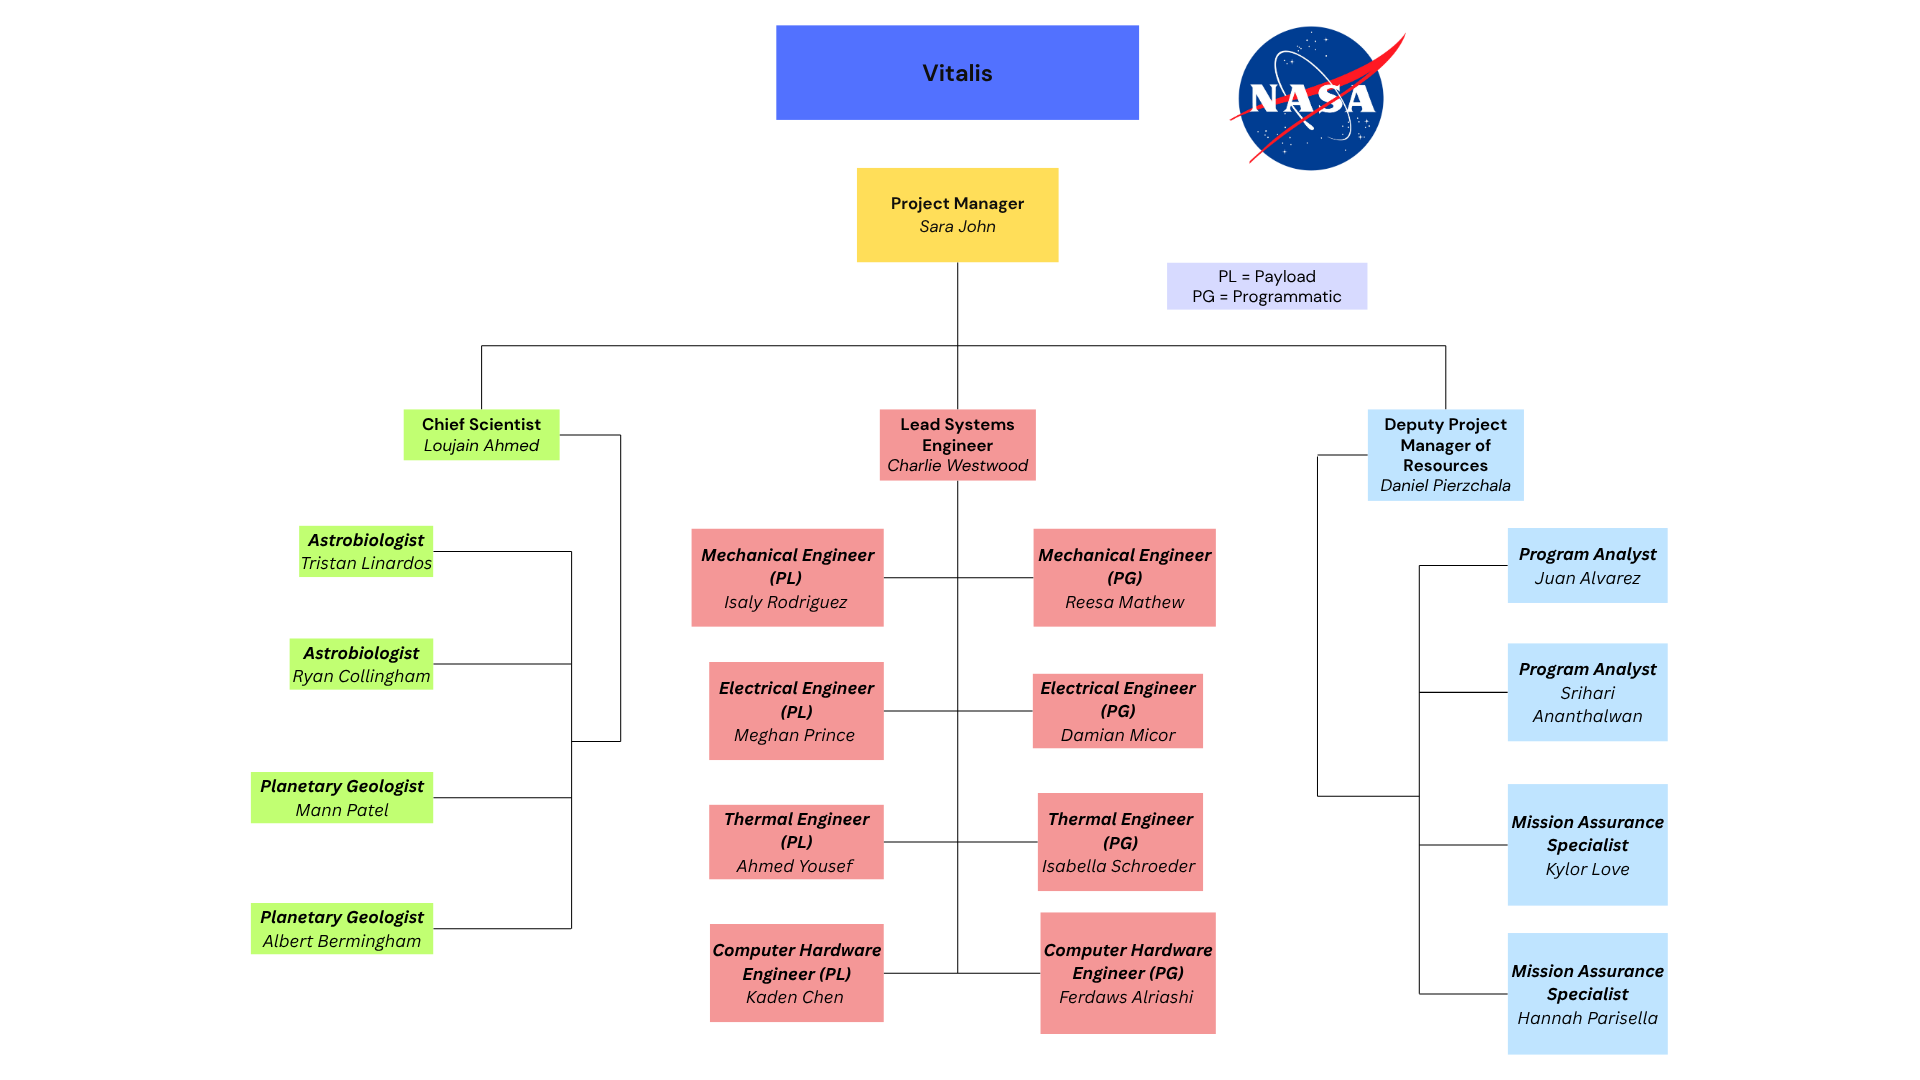
\includegraphics[width=1\textwidth]{images/orgchart.png}
    \caption{Team Organization Chart}
    \label{fig:orgchart}
\end{figure}

To help resolve some of the inevitable obstacles this mission will bring, the team will utilize varying methodologies depending on the technicality of the issue and allowable time. For technical issues, trade studies will be used to grade the solutions and system under criteria related to the mission to reveal which is optimal. For decisions which are time-sensitive or in an area which is not technical, those will be handled democratically. This style has the strength of allowing anyone to take the floor and present their ideas. This welcomes members of different specialties to bring out-of-the-box thinking and create unique solutions to potential problems. These ideas are voted upon with a majority choosing how to move forward. A democratic vote ensures participation from everyone, hence giving all a sense of ownership in the decision.\\

The likelihood of success in this endeavor is too early to be certain. As in these beginning stages all members are getting acquainted with their roles and responsibilities. The dynamics that this mission and its team are relatively unknown. Yet these shortcomings are only temporary as greater utilization of communication skills and resources are improving the team’s ability to meet deliverables daily. Many within the team plan to train with the skill modules, attend all related meetings, and read the handbooks offered. Once these habits are integrated with the team’s developing schedule system, success is assured.\\

\begin{table}[H]
\centering
\caption{Team’s Weekly Availability}
\label{tab:availability}
\begin{tabular}{|>{\raggedright}p{4cm}|>{\raggedright}p{6cm}|c|}
\hline
\textbf{Name} & \textbf{Role} & \textbf{Availability (hrs/week)} \\
\hline
Sara John & Project Manager & 8--10 \\
Daniel Pierzchala & Deputy Project Manager of Resources & 8--10 \\
Loujan Ahmed & Chief Scientist & 8--10 \\
Charlie Westwood & Lead Systems Engineer & 8--10 \\
Tristan Linardos & Astrobiologist & 4--6 \\
Ryan Collingham & Astrobiologist & 8--10 \\
Mann Patel & Planetary Geologist & 8--10 \\
Albert Bermingham & Planetary Geologist & 8--10 \\
Isaly Rodriguez & Mechanical Engineer (Payload) & 10+ \\
Meghan Prince & Electrical Engineer (Payload) & 6--8 \\
Ahmed Yousef & Thermal Engineer (Payload) & 8--10 \\
Kaden Chen & Computer Hardware Engineer (Payload) & 6--8 \\
Reesa Mathew & Mechanical Engineer (Programmatics) & 6--8 \\
Damian Micor & Electrical Engineer (Programmatics) & 4--6 \\
Isabella Schroeder & Thermal Engineer (Programmatics) & 8--10 \\
Ferdaws Alriashi & Computer Hardware Engineer (Programmatics) & 10+ \\
Juan Alvarez & Program Analyst & 8--10 \\
Srihari Ananthalwan & Program Analyst & 8--10 \\
Kylor Love & Mission Assurance Specialist & 6--8 \\
Hannah Parisella & Mission Assurance Specialist & 10+ \\
\hline
\end{tabular}
\end{table}
\subsection*{1.9.2 Schedule Basis of Estimate}
\addcontentsline{toc}{subsection}{1.9.3 Budget Basis of Estimate}

Following the completion of the Preliminary Design Review (PDR), the team will progress into creating a more detailed design, including additional subsystems and operational systems, collectively referred to as Phase C. Based on the timeline established for NASA’s \textit{Lucy Mission}, which had a similar budget and duration for Pre-Phase A, Phase A, and Phase B tasks—assumed to have already been completed—the team should be allotted one year to complete Phase C. Therefore, the expected date of completion and approval for the Critical Design Review (CDR) is August 19, 2026. Key Decision Point (KDP) meetings are assumed to occur over a five-day period, shortly before the end of Phases C, D, and E. These meetings will be held at NASA Headquarters in Washington, D.C.

Upon CDR approval, the project will enter Phase D, which includes system assembly, manufacturing, integration, testing, and launch preparation. Using the \textit{Lucy Mission} as a reference, Phase D will begin by June 2027. The team will utilize the preceding year for preparations, including materials acquisition, team coordination, and subsystem prototyping. The rover system must be fully integrated and ready by October 1, 2029, aligning with constraints outlined in the Mission Task Document provided by NASA L’SPACE.

A two-month buffer will be allocated for risk mitigation and final verifications. Launch readiness is set for December 1, 2029. In preparation, the team will travel to Orlando, Florida for a five-day window surrounding launch—arriving two days before and departing two days after.

Following launch, the mission enters Phase E. Based on the transit duration of the \textit{Opportunity Rover}, a seven-and-a-half-month cruise phase is expected before Mars arrival. Upon successful landing, the rover will begin surface operations and data collection over the course of 15 Earth years. The data collected will be transmitted back to Earth and analyzed through 2044. These findings are expected to significantly advance our understanding of Martian hydrology and geology, ultimately supporting future human exploration initiatives.
\subsection*{1.9.3 Budget Basis of Estimate}
\section*{1.10 Conclusion}
\addcontentsline{toc}{section}{1.10 Conclusion}
\clearpage

%use the chicage style

\bibliography{refs}
\clearpage
\section*{Declaration of Generative AI Use in the Writing Process}
\addcontentsline{toc}{section}{Declaration of Generative AI Use in the Writing Process}

During the preparation of this work, the team used \textbf{ChatGPT (OpenAI)} to assist with the drafting, formatting, and refinement of several textual components of the Mission Concept Review (MCR) document. Specifically, ChatGPT was used in:

% Add any other ways people on the team used gen AI 
\begin{itemize}
    \item \textbf{LaTeX Formatting and Table of Contents Integration:} Aided in generating consistent LaTeX code for section headers, tables, and figure placement across the document.
\end{itemize}

After using this tool, the team thoroughly reviewed and edited the content to ensure accuracy, technical validity, and originality. The team takes full responsibility for the final content of the deliverable.



\clearpage
\section*{Appendix}
\addcontentsline{toc}{section}{Appendix}

\begin{table}[H]
\centering
\caption{TBD/TBR Resolution Plan}
\renewcommand{\arraystretch}{1.6}
\small
\begin{tabular}{|c|p{13cm}|}
\hline
\textbf{TBD / TBR \#} & \textbf{Plans and Timeline for Resolution} \\
\hline
1 & Parameters to be determined by June 30th, 2025. \\
2 & Values to be determined by June 30th, 2025. \\
3 & Parameters to be determined by June 30th, 2025. \\
4 & Values to be determined by June 30th, 2025. \\
5 & Instrument performance to be predicted by June 30th, 2025. \\
6 & Instrument to be determined by June 30th, 2025. \\
7 & Instrument performance to be predicted by June 30th, 2025. \\
8 & Instrument to be determined by June 30th, 2025. \\
9 & Mission requirements to be determined by June 30th, 2025. \\
10 & Mission requirements to be determined by June 30th, 2025. \\
\hline
\end{tabular}
\end{table}

\end{document}